\PassOptionsToPackage{svgnames}{xcolor}
\documentclass[10pt,letterpaper]{article}
\usepackage[top=.5in, bottom=.75in, left=.5in, right=.5in]{geometry}
\usepackage{tcolorbox}
\usepackage{lipsum}
\tcbuselibrary{skins,breakable}
\usetikzlibrary{shadings,shadows}

\usepackage{graphicx} % Allows to include images
\usepackage{booktabs} % Allows the use of \toprule, \midrule and \bottomrule in tables

\usepackage{multicol}
\usepackage{float}

\usepackage[T1]{fontenc}
\usepackage[utf8]{inputenc}
\usepackage{lmodern}

\title{\vspace{-.5in}Practice 4: Master Dribbling}
\author{\vspace{-.5in}}
\date{\vspace{-.5in}}

\newenvironment{agendablock}[1]{%
    \tcolorbox[beamer,%
    noparskip,breakable,
    colback=LightGray,colframe=Black,%
    colbacklower=Gray!75!LightGray,%
    title=#1]}%
    {\endtcolorbox}

\newenvironment{evenBlock}[1]{%
    \tcolorbox[beamer,%
    noparskip,breakable,
    colback=LightGreen,colframe=DarkGreen,%
    colbacklower=LimeGreen!75!LightGreen,%
    title=#1]}%
    {\endtcolorbox}

\newenvironment{oddBlock}[1]{%
    \tcolorbox[beamer,%
    noparskip,breakable,
    colback=LightBlue,colframe=DarkBlue,%
    colbacklower=DarkBlue!75!LightBlue,%
    title=#1]}%
    {\endtcolorbox}

\newenvironment{myexampleblock}[1]{%
    \tcolorbox[beamer,%
    noparskip,breakable,
    colback=LightGreen,colframe=DarkGreen,%
    colbacklower=LimeGreen!75!LightGreen,%
    title=#1]}%
    {\endtcolorbox}

\newenvironment{myalertblock}[1]{%
    \tcolorbox[beamer,%
    noparskip,breakable,
    colback=LightCoral,colframe=DarkRed,%
    colbacklower=Tomato!75!LightCoral,%
    title=#1]}%
    {\endtcolorbox}

\newenvironment{myblock}[1]{%
    \tcolorbox[beamer,%
    noparskip,breakable,
    colback=LightBlue,colframe=DarkBlue,%
    colbacklower=DarkBlue!75!LightBlue,%
    title=#1]}%
    {\endtcolorbox}

\begin{document}

\fontfamily{lmss}\selectfont

\maketitle

\begin{agendablock}{Practice Activities}
    Dribbling and Ball Control at your feet is another key skill.  The ability to dribble well allows you to find open space to pass or shoot. 
    \begin{enumerate}
        \item Warm ups / Coerver Touches, HowTo [ 20 min ]
        \item Drills [ 30 min ]
        \item Game Situational Drills [ 15 min ]
        \item Small Sided Game [ 20 min ]
        \item Sprints [ 5 min ]
    \end{enumerate}
\end{agendablock}

\section{Warm Ups}
Run the \textbf{GATE DRIBBLING} drill until everyone arrives and for a few minutes after.

\textbf{Time: 2 minutes}
\begin{oddBlock}{Gate Dribbling}
Setup 2-4 square areas about 6x6 yards.  Then add one of each colored gate to the squares (ideally 4 gates per square each a different color).  The cones for each gate should be about a yard apart.  The goal is to have the players dribble through the each colored gate in each zone once.  First one to complete all gate in each zone wins.
\end{oddBlock}

\textbf{Time: 3 minutes}
\begin{myalertblock}{Theme of the Practice}
    \textbf{Perfect Dribbling!}

    Importance of Dribbling:
    \begin{itemize}
        \setlength{\itemsep}{0pt}
        \setlength{\parskip}{0pt}
        \setlength{\parsep}{0pt}
        \item Dribbling sets up everything.
        \item Creates space to pass.
        \item Creates space to shoot.
        \item No offsides.
        \item Can attract or freeze defenders to allow yuor teammates to find open space.
    \end{itemize}

    Issues with Dribbling:
    \begin{itemize}
        \setlength{\itemsep}{0pt}
        \setlength{\parskip}{0pt}
        \setlength{\parsep}{0pt}
        \item Dribbling moves the ball slower than passing or running.
        \item Attracts defenders (can be a positive - see above).
    \end{itemize}

\end{myalertblock}

\textbf{Time: 10 minutes}
\begin{agendablock}{Captain Led Warm ups / Coerver Touches (15 min) }
    \textbf{Warmups}
    \begin{enumerate}
        \item Jog to the 18 yard line and back twice with your ball (inside cut first time, outside cut the second),
        \item Side-Step to 18 yd line and back twice,
        \item Butt Kickers to the 18 yd line and back twice,
        \item Jog Backwards to the 18 yd line and back twice.
    \end{enumerate}
    \textbf{Touches}
    \begin{enumerate}
        \item Toe-Touches (20 count alternating feet).
        \item Pull back and Push Forward (10 each foot).
        \item Side to Side or Pendulums (20 count).
        \item Triangles (10 each foot).
        \item Pullback-Behind (20 count).
    \end{enumerate}
\end{agendablock}

\section{HOWTO:}
\begin{evenBlock}{HOWTO:  Dribble (5 min)}

\begin{minipage}[t]{\linewidth}
    \centering
    Review these elements prior to beginning the dribbling drills so its fresh in their heads.

    %\begin{minipage}{.3\linewidth} % Left column and width
        %\centering
        %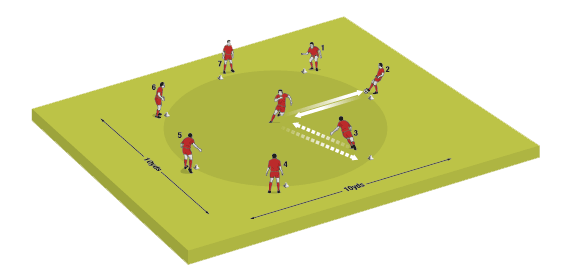
\includegraphics[width=\textwidth]{../img/Trimmed/Clocks1}
    %\end{minipage}
    %\hspace{0.05\linewidth}
    %\begin{minipage}{.6\linewidth} % Left column and width
    
        \textbf{Methods of Dribbling:}
        \begin{enumerate}
        \setlength{\itemsep}{0pt}
        \setlength{\parskip}{0pt}
        \setlength{\parsep}{0pt}
        \item Inside of the foot - used for control, turning.
        \item Outside/Laces of the foot - used for speed and balance.
        \end{enumerate}
        
        Demonstrate running with inside of foot facing forward vs. running with outside or laces forward.

        Have the boys try running both ways and ask which methods allows them to run faster?

    %\end{minipage}
\end{minipage}

\end{evenBlock}

\section{Drills}

\textbf{Time: 10 minutes}
\begin{evenBlock}{Cone Weave Dribbling (10 min)}


\begin{minipage}[t]{\linewidth}
    \centering
    
    \begin{minipage}{.3\linewidth} % Left column and width
        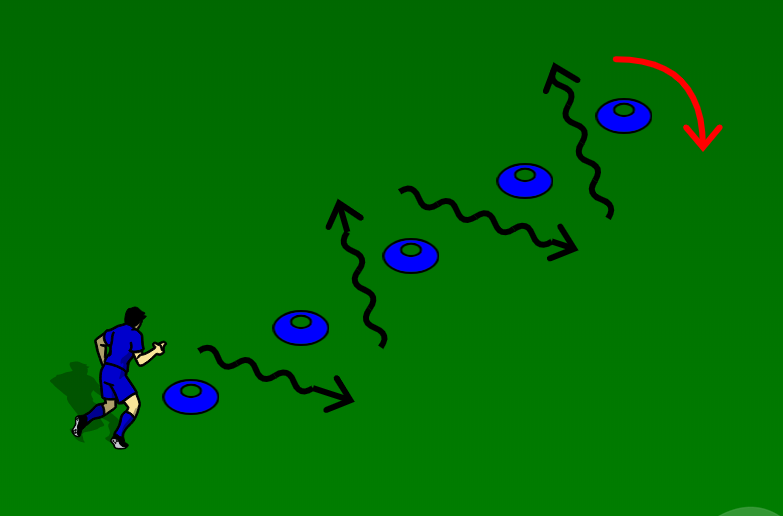
\includegraphics[width=\textwidth]{../img/Trimmed/cone_dribbling}
    \end{minipage}
    \hspace{0.05\linewidth}
    \begin{minipage}{.6\linewidth} % Left column and width
        \textbf{Drill Description:}
        Dribble around 6 cones about 1 yard apart, using only the inside portion of the foot to make cuts.  Ends are different color, orange inside cut, green outside cut.  Players should focus on using 3 touches to make the turn around the end cones.

        \vspace{3pt}
        
        Advanced - use only the outside of the foot or alternate inside foot one direction, outside foot when traveling the other direction.
        %\end{enumerate}

        \vspace{10pt}
        
        \textbf{Coaching Points:}
        \begin{itemize}
        \setlength{\itemsep}{0pt}
        \setlength{\parskip}{0pt}
        \setlength{\parsep}{0pt}
        \item Go slow at first and work up speed as control increases.
        \item Control should be the focus of this drill.  As control increases, increase speed.
        \item Players should always be on their toes, no standing flat footed.
        \item Its better to have 3-5 small controlled touches around the last cone than 3 large out of control touches.
        \end{itemize}

    \end{minipage}
\end{minipage}

\end{evenBlock}

\textbf{Time: 10 minutes}
\begin{oddBlock}{Straight line dribbling at speed ( 10 min )}
    \textbf{Drill:}
    \begin{enumerate}
        \setlength{\itemsep}{0pt}
        \setlength{\parskip}{0pt}
        \setlength{\parsep}{0pt}
        \item Use the outside of the foot or laces to push the ball forward 2-3 steps in front of you.
        \item Continue until half field then make a turn inside cut and back to the end line.
    \end{enumerate}
    \textbf{Coaching Points:}
    \begin{enumerate}
        \setlength{\itemsep}{0pt}
        \setlength{\parskip}{0pt}
        \setlength{\parsep}{0pt}
        \item Go slow until and get used to the feel of dribbling this way.
        \item Increase speed as it begins to feel more natural.
        \item Focus on your touch and timing as you approach the lines and try to make that cut right on the line.
        \item Can you beat coach?
    \end{enumerate}
\end{oddBlock}

\textbf{Time: 10 minutes}
%\begin{evenBlock}{Gate Dribbling (10 min)}
%Set up 3 gates in a zig-zag pattern about 6 to 10 yards apart.  The gates should be about a yard wide or less depending on dribbling skill of the group.  Players start a the end line and dribble through the gates as fast as possible.  Use the same technique as the previous drill.
%\end{evenBlock}

\begin{oddBlock}{Gate Dribbling (10 min)}

\begin{minipage}[t]{\linewidth}
    \centering
    
    \begin{minipage}{.3\linewidth} % Left column and width
        %\begin{figure}
            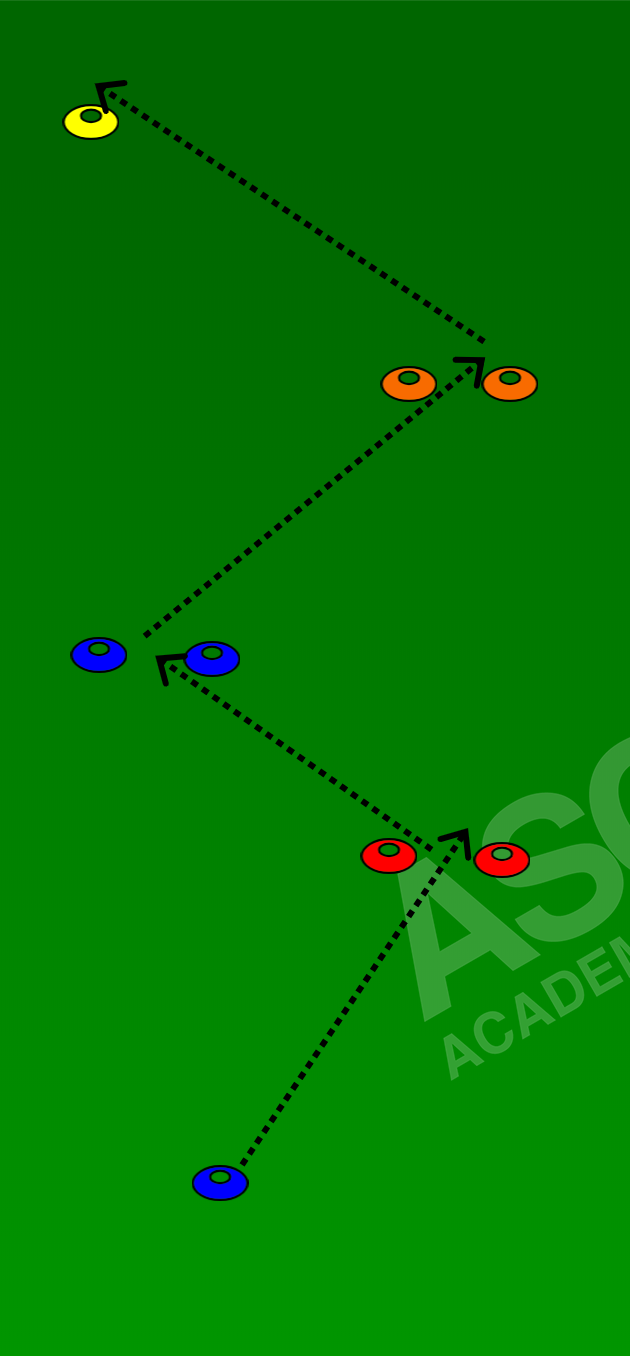
\includegraphics[width=.6\textwidth]{../img/Trimmed/Gate_Dribbling}
        %    \caption{Drill: 4 Person Passing}
        %\end{figure}
    \end{minipage}
    \hspace{0.05\linewidth}
    \begin{minipage}{.6\linewidth} % Left column and width
        \textbf{Drill Description:}
        The object is to dribble at full speed through 3 narrow gates set in a zig-zag pattern about 6 to 10 yards apart.  The gates should be about a yard wide or less depending on dribbling skill of the group.  Once they explode past the yellow cone, they jog back to the end of the line.  Use speed dribbling technique.
        \begin{enumerate}
        \setlength{\itemsep}{0pt}
        \setlength{\parskip}{0pt}
        \setlength{\parsep}{0pt}
        \item Players start at blue gate
        \item Then dribble the ball through the gates.
        \item Once they dribble through the orange gate they explode past the yellow cone.
        \item Then jog back to the end of the line.
        \end{enumerate}

        \textbf{Coaching Points:}
        \begin{itemize}
        \setlength{\itemsep}{0pt}
        \setlength{\parskip}{0pt}
        \setlength{\parsep}{0pt}
        \item When first starting, it will help to focus on proper technique over speed.  Increase the speed as the their technique improves.
        \item Technique uses top outside of the foot, toe down, pushing the ball forward 2 or 3 steps.
        \item Set width of of the gate based on skill.
        \end{itemize}

    \end{minipage}
\end{minipage}

\end{oddBlock}


\section{Game Situational Practice}
\textbf{Time: 15 minutes, Started by 6:20PM}
\begin{evenBlock}{Endzone Soccer (Dribble)}
\textbf{Goal:} Learn to recognize open space and how to attack that open space and beat a defender.  Learn to know when to pass as defensive pressure builds around you.
\begin{minipage}[t]{\linewidth}
    \begin{minipage}{.3\linewidth} % Left column and width
        \centering
        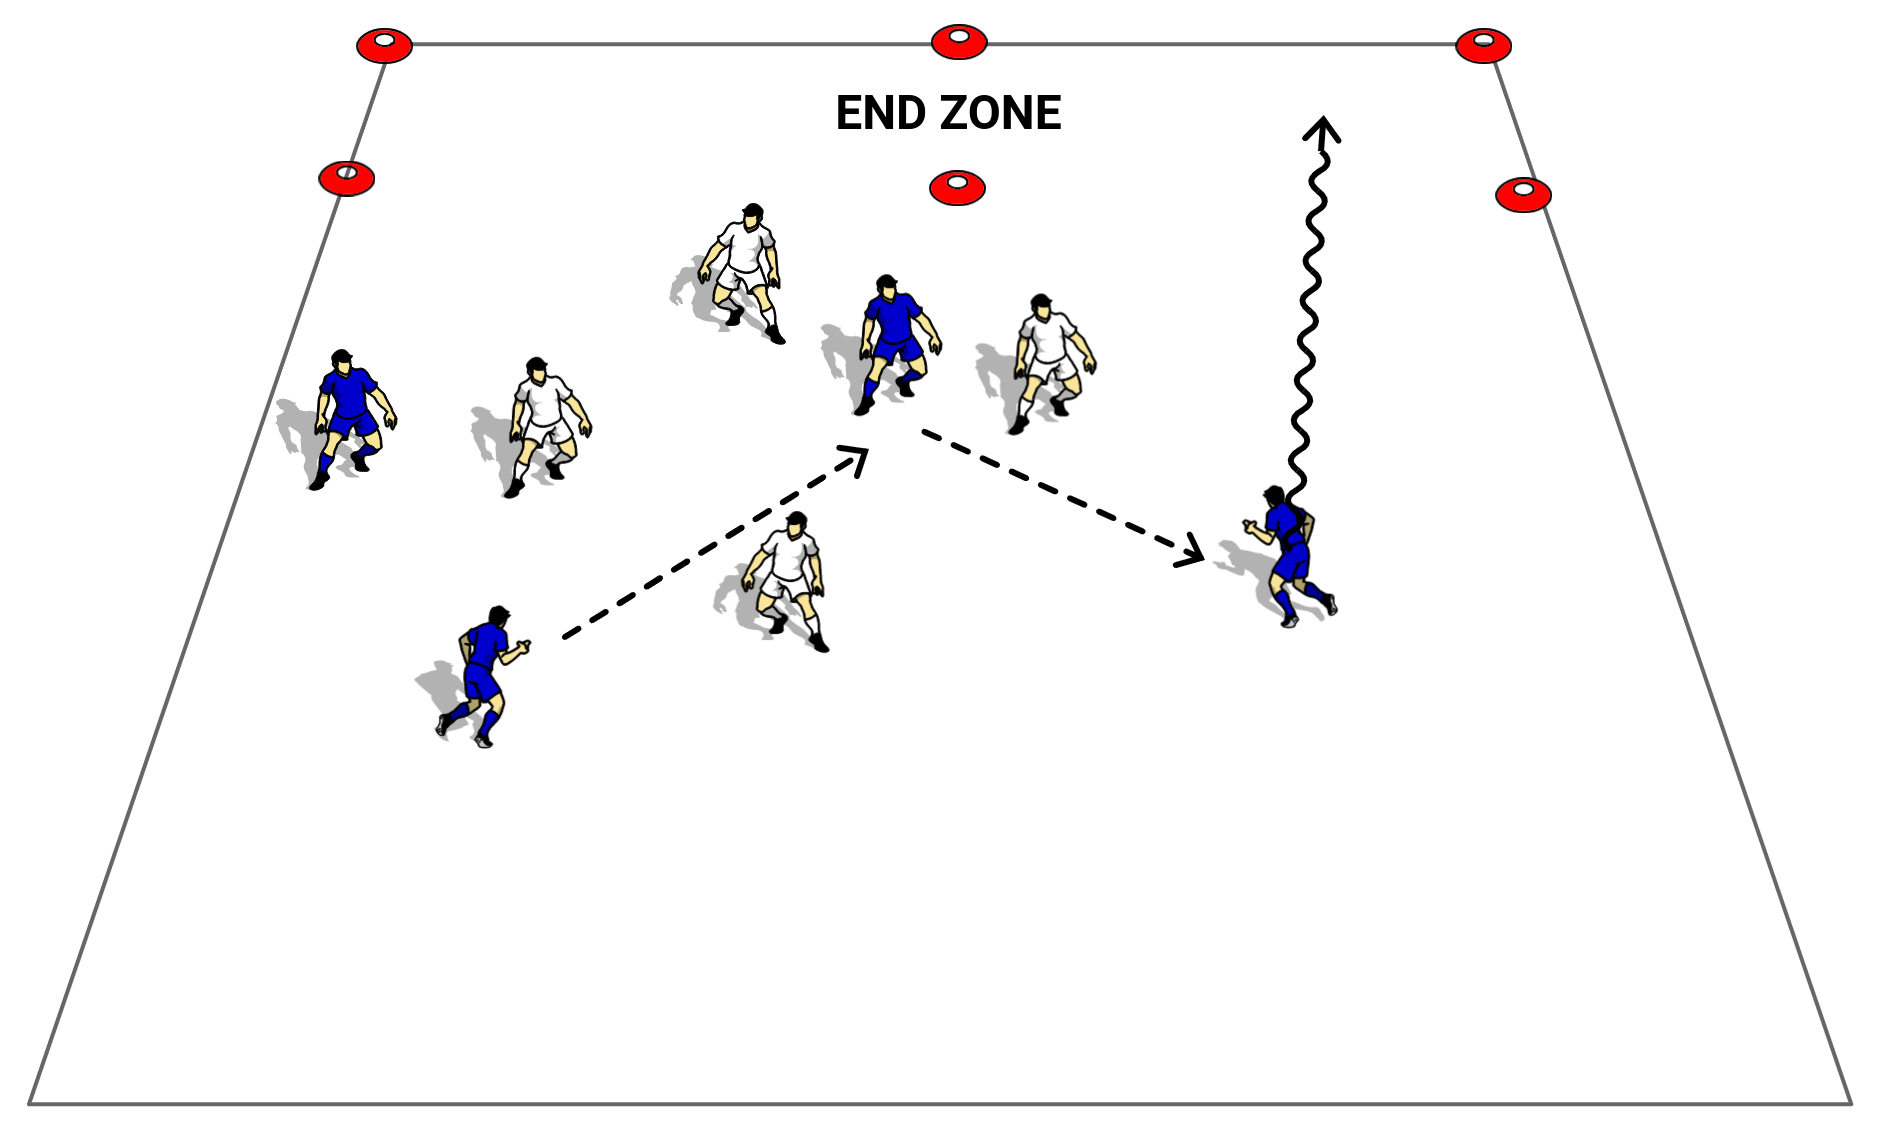
\includegraphics[width=\textwidth]{../img/Trimmed/EndZoneSoccer_DribbleScore}
    \end{minipage}
    \hspace{0.05\linewidth}
    \begin{minipage}{.6\linewidth} % Left column and width
        \textbf{Drill Description:}
        \begin{enumerate}
            \setlength{\itemsep}{0pt}
            \setlength{\parskip}{0pt}
            \setlength{\parsep}{0pt}
            \item 4v4 Small sided activity.
            \item The goal is to dribble the ball into the end zone under control and stop the ball.
            \item Only the person with the ball can enter the end zone unless the defender is backed into the endzone by the attacking player.
            \item Once the ball is stopped in the endzone that team scores and the other team gets the ball at the top.
            \item If the defending team steals the ball they become the attackers but must pass the ball at least once before entering the endzone.
            \item Any out of bounds plays result in the defending team winning the ball, unless the defending team kicks the ball out the back of the end zone.
            \item If the attacking team passes the ball into the endzone the ball is dead and awarded to the defending team.
        \end{enumerate}
    \end{minipage}
\end{minipage}
\raggedright
    \textbf{Coaching Points:}
    \begin{itemize}
        \setlength{\itemsep}{0pt}
        \setlength{\parskip}{0pt}
        \setlength{\parsep}{0pt}
        \item Look to exploit open space in front or behind the defender.
        \item Use and try moves to beat the defender.
        \item Learn how to time these moves, usually they need to happen sooner than one thinks.
        \item Learn to feel the defensive pressure and passing to an open teammate.
        \item Learn to keep your head up and find an open player.

    \end{itemize}

\end{evenBlock}

%\begin{evenBlock}{Outside Forward Drive to Endline and Cross (10 min)}

\begin{minipage}[t]{\linewidth}
    \centering
    
    \begin{minipage}{.3\linewidth} % Left column and width
        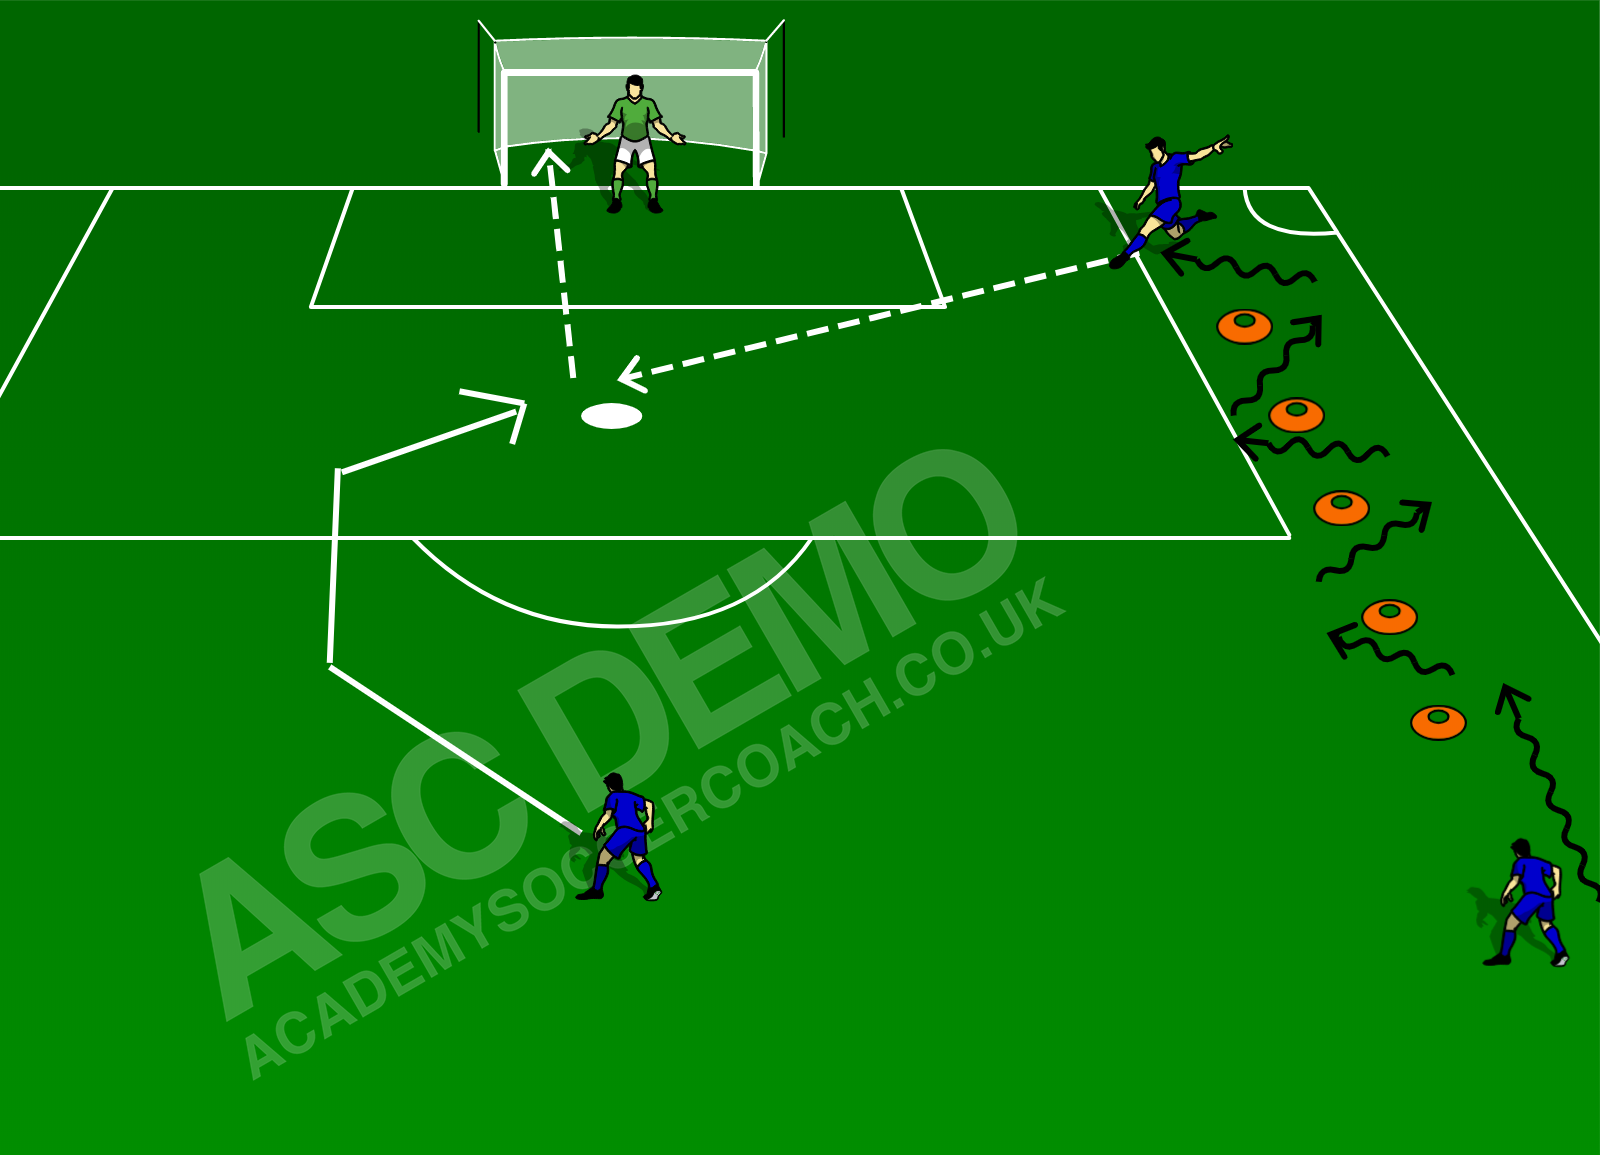
\includegraphics[width=\textwidth]{../img/Trimmed/Dribble-Cross-Shoot}
    \end{minipage}
    \hspace{0.05\linewidth}
    \begin{minipage}{.6\linewidth} % Left column and width
        \textbf{Drill Description:}
        \begin{enumerate}
        \setlength{\itemsep}{0pt}
        \setlength{\parskip}{0pt}
        \setlength{\parsep}{0pt}
        \item A line forms at half field, with a set of balls.
        \item Player 1 dribbles through cones, turning around the last cone toward goal,
        \item P1 then crosses the ball to the PK spot where the Striker takes his one touch shot.
        \item Striker retrieves the ball and goes to the end of the line.
        \item Wing then shifts to the striker role.
        \end{enumerate}

        \vspace{6pt}
        
        Once everyone goes once or twice switch side of the field and uses left feet for crossing and shooting.

        \vspace{6pt}
        
        Playing a Keeper is optional.

        \vspace{10pt}
        
        \textbf{Coaching Points:}
        \begin{itemize}
        \setlength{\itemsep}{0pt}
        \setlength{\parskip}{0pt}
        \setlength{\parsep}{0pt}
        \item The touch around that last cone is the most important. 
        \item Body position around that last cone is critical as well.  The players hips need to be tuned toward the PK spot otherwise the player gives up both power and control over the pass.
        \item The striker must be patient and not over run the spot.  Move in an arc away from center, then back toward the ball.  Accelerate once the ball is passed and kick it into goal.
        \end{itemize}

    \end{minipage}
\end{minipage}

\end{evenBlock}

%\begin{evenBlock}{2 vs. 1 Offense (10 min)}


\begin{minipage}[t]{\linewidth}
    \centering
    
    \begin{minipage}{.3\linewidth} % Left column and width
        %\begin{figure}
            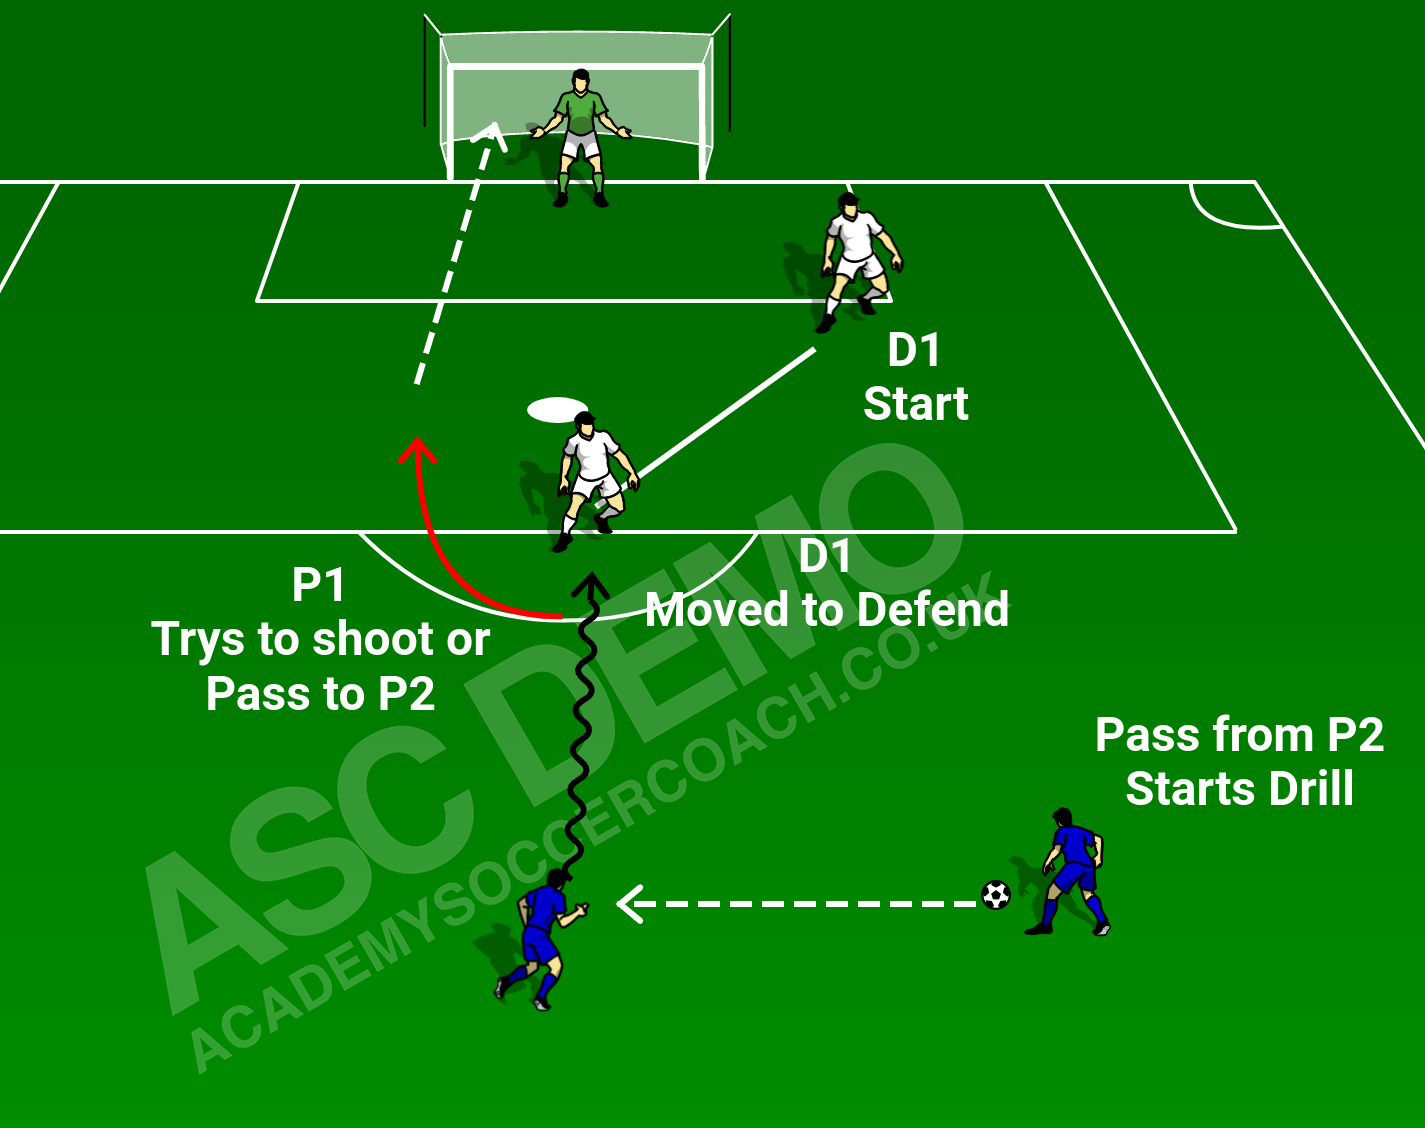
\includegraphics[width=\textwidth]{../img/Trimmed/2v1_Option}

            \vspace{3pt}
            
            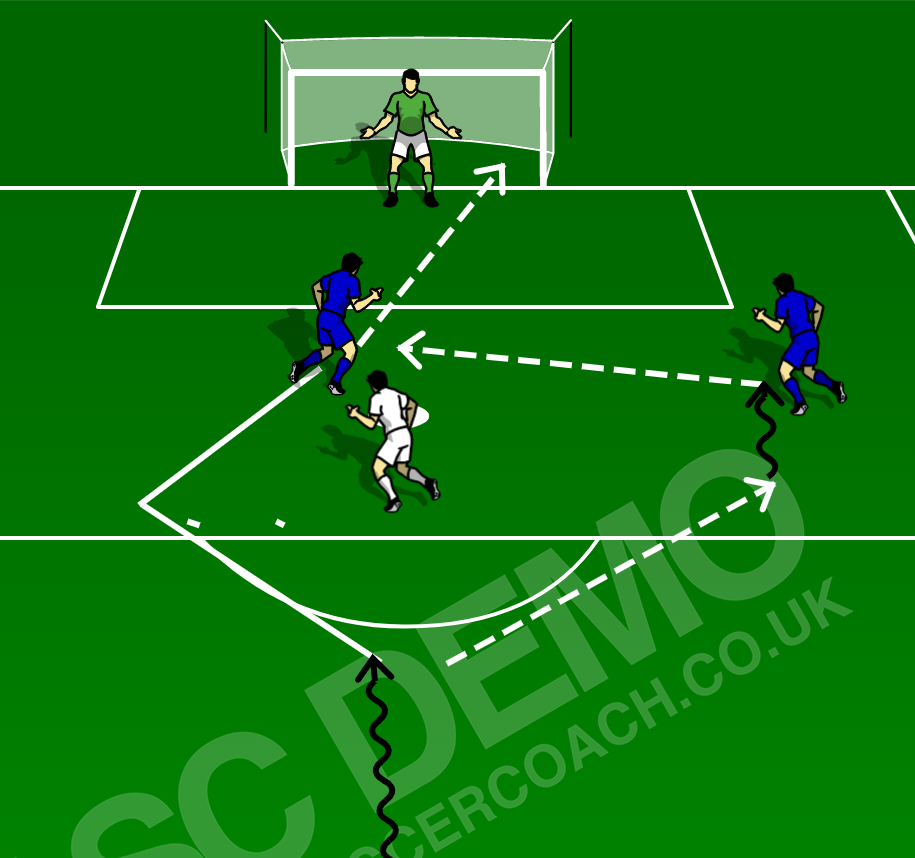
\includegraphics[width=\textwidth]{../img/Trimmed/2v1_Option_Pass}
        %    \caption{Drill: 4 Person Passing}
        %\end{figure}
    \end{minipage}
    \hspace{0.05\linewidth}
    \begin{minipage}{.6\linewidth} % Left column and width
        \textbf{Drill Description:}
        This drill is designed train the forward to make a quick decision on how to beat a defender.  He has two options, dribble around the defender or pass to his wing and make a move around the defender. 
        \begin{enumerate}
        \setlength{\itemsep}{0pt}
        \setlength{\parskip}{0pt}
        \setlength{\parsep}{0pt}
        \item The wing (P2) starts the play by passing to the forward.  The defender (D1) starts at the corner of the 6 yard box.
        \item The forward drives to goal as a defender come charging to defend.
        \item The forward has two choices, pass or make a move/touch around the defender.
        \item The goal is to get a shot on goal.
        \item If he passes the ball, the wing should cross the ball quickly as the striker is passing the defender.
        \end{enumerate}

        \vspace{3pt}
        
        Rotate rolls each shot: P2 to P1, P1 to D1, D1 to P2.

        \vspace{10pt}
        
        \textbf{Coaching Points:}
        \begin{itemize}
        \setlength{\itemsep}{0pt}
        \setlength{\parskip}{0pt}
        \setlength{\parsep}{0pt}
        \item The forward needs to decide quickly which option he plans to take.
        \item The wing needs to be ready at all times and should stay `on-side'.
        \item The forward should try and take advantage of any weakness of the defense, or try and create weakness by using a scissor move or a fake.
        \item Explain on-sides and off-sides.
        \end{itemize}

    \end{minipage}
\end{minipage}

\end{evenBlock}

\section{Game}

\begin{oddBlock}{Small Sided}
    \textbf{Start Time: 6:35 PM}
    \textbf{Time:} 10 minute halves.

    \textbf{Size:} 4v4 or 5v5.

    Express:
    \begin{itemize}
        \setlength{\itemsep}{0pt}
        \setlength{\parskip}{0pt}
        \setlength{\parsep}{0pt}
        \item  remind them about the practice: dribble into open space,
        \item dribble to pull defenders away from teammates,
        \item Look to beat a defender and shoot or pass.
        \item Funnel Positioning.
        \item Go outside on our defensive half.
        \item Pass quickly down sidelines or into open space.
        \item Avoid passing backward.
        \item Make a pass early or move early.
    \end{itemize}

\end{oddBlock}

\section{Close}
\begin{oddBlock}{Sprints}
    Escalation sprints while dribbling, sprint dribble to 15 yards and back, 30 yards and back, 45 yards and back, then 60 yards and back.

    \vspace{12pt}
    
    Slowly dribble around the border of the 19 yard box to cool down.

\end{oddBlock}

\end{document}